
\chapter{Experiment and Result}
brief of experiment and result.
\section{Experiment}
Please tell how the experiment conducted from method.

\section{Result}
Please provide the result of experiment

\section{Mhd Zulfikar Akram Nastuion / 1164081}
\subsection{Teori}
\begin{enumerate}
\item Klasifikasi Teks
\par
Klasifikasi teks adalah sebuah proses untuk menempatkan dokumen teks ke dalam suatu kategori berdasarkan isi dari teks tersebut. 
\item Kenapa klasifikasi bunga tidak bisa menggunakan machine learning
\par
Klasifikasi bunga tidak dapat digunakan pada machine learning karena terdapat masalah, yaitu apabila kita memasukkan suatu inputan yang sama tetapi outputnya berbeda.
\item  Teknik pembelajaran mesin pada teks pada kata-kata yang digunakan di Youtube
\par
Penggunaan machine learning pada Youtube contohnya ada pada saat kita sedang melakukan pencarian judul, nama dan lainnya maka youtube akan menampilkan apa yang kita cari, kemudian saat kita sedang melihat youtube, dibagian kanan video terlihat ada tampilan video yang berkaitan dengan apa yang kita cari atau kita ketikkan di tempat pencarian terbebut.
\item Vectorisasi Data
\par
Vektorisasi data adalah sebuah proses pembagian dan pemecahan data kemudian dilakukan perhitungan datanya.
\item Bag of Words
\par
Bag of words adalah sebuah proses penyederhanaan yang digunakan dalam pengambilan informasi.
\item TF-IDF
\par
TF-IDF adalah sebuah metode untuk menghitung beberapa kata yang muncul dari setiap kata yang paling umum digunakan.
\end{enumerate}

\subsection{Praktek}
\begin{enumerate}
\item Membuat aplikasi sederhana meggunakan pandas
\begin{figure}[ht]
\centering
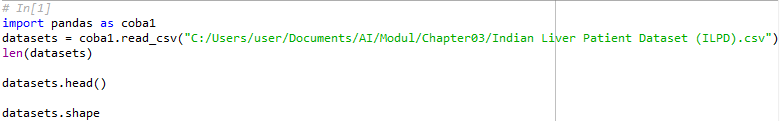
\includegraphics[scale=0.7]{figures/pandas/4_1.png}
\caption{Aplikasi sederhana pandas}
\end{figure}
\begin{itemize}
\item Baris 1: Memanggil library pandas sebagai coba1
\item Baris 2: Membaca dataset Indian Liver Patient Dataset
\item Baris 3: Dataset.head menampilkan jumlah baris pada dataset
\item Baris 4: Dataset.shape menampilkan jumlah kolom pada dateset
\par Hasilnya seperti gambar 4.1
\end{itemize}
\item Membuat aplikasi sederhana meggunakan pandas
\begin{figure}[ht]
\centering
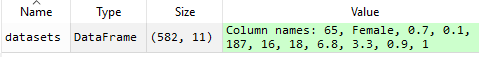
\includegraphics[scale=0.9]{figures/pandas/4_2.png}
\caption{Hasil aplikasi sederhana pandas}
\end{figure}
\item Membuat aplikasi sederhana menggunakan pandas, dan membuat data dummy sebanyak 500 baris dan melakukan data load ke data frame panda
\begin{figure}[ht]
\centering
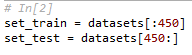
\includegraphics[scale=0.9]{figures/pandas/4_3.png}
\caption{Membuat data dummy sebanyak 500}
\end{figure}
\begin{itemize}
\item Baris 1: Membagi data set ILPD dari 500 data menjadi data train menjadi 450 data.
\item Baris 2: Membagi data set ILPD dari sisa pembagian data train menjadi data test menjadi 50 data.
\end{itemize}
\par Hasilnya seperti pada gambar 4.3
\begin{figure}[ht]
\centering
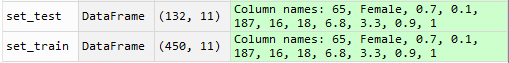
\includegraphics[scale=0.9]{figures/pandas/4_4.png}
\caption{Hasil membuat data dummy sebanyak 500}
\end{figure}
\item  Vektorisasi dan Klasifikasi Data Dengan Decission Tree
\begin{itemize}
\item Berikut ini adalah hasil dari NPM mod 4
\end{itemize}
\begin{figure}[ht]
\centering
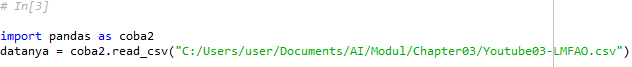
\includegraphics[scale=0.9]{figures/pandas/4_5.png}
\caption{NPM mod 4}
\end{figure}
\begin {itemize}
\item Vektorisasi seperti pada gambar 4.4
\end{itemize}
\begin{figure}[ht]
\centering
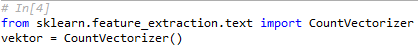
\includegraphics[scale=0.9]{figures/pandas/4_6.png}
\caption{Vektorisasi}
\end{figure}
\begin {itemize}
\item Klasifikasi data dengan desision Tree seperti pada gambar 4.5
\end{itemize}
\begin{figure}[ht]
\centering
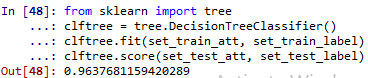
\includegraphics[scale=0.7]{figures/pandas/4_7.png}
\caption{Klasifikasi dengan Tree}
\end{figure}
\begin{itemize}
\item Dalam in 48 impor tree dari sklearn. Dan mendefinisikan variabel clftree untuk memanggil Decission Tree Classifier dan melakukan fit atau pengujian.
\item clftree.score memunculkan akurasi prediksi yang dilakukan terhadap clftree
\end{itemize}
\item Klasifikasi SVM seperti pada gambar 4.6
\begin{figure}[ht]
\centering
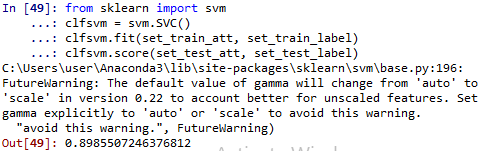
\includegraphics[scale=0.9]{figures/pandas/4_8.png}
\caption{Klasifikasi SVM}
\end{figure}
\begin{itemize}
\item Import SVM dari  sklearn
\item Melakukan fit dari train att dan train label atau disebut denga pengujian
\item Mendefinisikan variabel clfsvm untuk melakukan prediksi dataset Youtube LMFAO dengan SVM. Dan akan muncul hasil prediksinya 
\end{itemize}
\item Klasifikasi decision tree seperti pada gambar 4.7
\begin{figure}[ht]
\centering
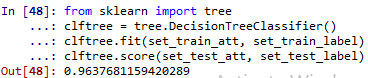
\includegraphics[scale=0.9]{figures/pandas/4_7.png}
\caption{Klasifikasi decision tree}
\end{figure}
\begin{itemize}
\item Import tree dari  sklearn
\item Melakukan fit dari train att dan train label atau disebut denga pengujian
\item  clftree.score memunculkan akurasi prediksi yang dilakukan terhadap clftree 
\end{itemize}
\item Matplotlib seperti pada gambar4.8
\begin{figure}[ht]
\centering
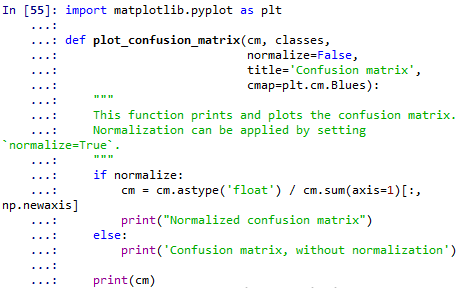
\includegraphics[scale=0.9]{figures/pandas/4_9.png}
\caption{Matplotlib}
\end{figure}
\par Fungsi ini mencetak dan memplot Confussion Matrix. Normalisasi dapat diterapkan dengan mengatur `normalize = True`. Ada Confussion Matrik menggunakan normalisasi dan ada confussion matrik tidak menggunakan normalisasi.
\item Menjelaskan program cross validation seperti pada gambar 4.9
\begin{figure}[ht]
\centering
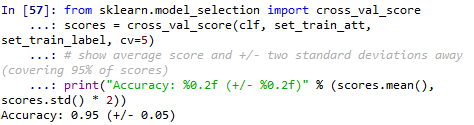
\includegraphics[scale=0.9]{figures/pandas/4_10.png}
\caption{Cross Validation}
\end{figure}
\par Variable score akan melakukan cross validation pada variable clf, train att, train label. Variabel scores akan menghitung nilai rata-rat menggunakan function mean. Dan scores menghitung standar deviasi dari data yang diberikan. Hasilnya seperti pada gambar 4.10
\begin{figure}[ht]
\centering
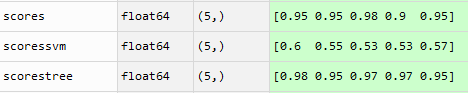
\includegraphics[scale=0.9]{figures/pandas/4_11.png}
\caption{Hasil Cross Validation}
\end{figure}
\item Proses pengamatan komponen seperti pada gambar 4.11
\begin{figure}[ht]
\centering
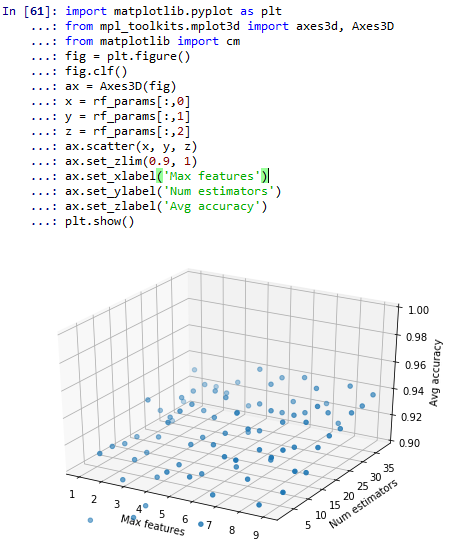
\includegraphics[scale=0.9]{figures/pandas/4_12.png}
\caption{Pengamatan komponen}
\end{figure}
\par Pada gambar tersebut merupakan kodingan dan hasil dari macfeatures, num estimators dan accuracy.
\end{enumerate}